% NOTE: this .tex file is in subdirectory 'examples'. You need to move it
% up to project root before attempting to compile (and adjust all 
% in-document links to include the subdirectory). Alternatively,
% move class and related files down into this directory.
%
%% Select the dissertation mode on
%
% See the documentation for more information about the available class options 
% ('math', 'vertlayout', 'pdfa', ...)
% If you give option 'draft' or 'draft*', the draft mode is turned on
% NOTE if you want to generate abstracts for the publication platform, use
% the option 'abstracts'!
% The pdfa option is experimental, but give it a try -- your doc will be better archivable
%
\documentclass[dissertation,math,vertlayout,pdfa,colorlinks,nologo]{aaltoseries}

% Kludge to make sure we have utf8 input (check that this file is utf8!)
\makeatletter
\@ifpackageloaded{inputenc}{%
  \inputencoding{utf8}}{%
  \usepackage[utf8]{inputenc}}
\makeatother

% for live links. Takes the above option 'colorlinks' (use 'hidelinks' if you want them black for print).
\usepackage{hyperref} 

% Lipsum package generates quasi latin filler text
\usepackage{lipsum}
% Set the document languages used
\usepackage[finnish,swedish,english]{babel}
% more math symbols and environments if needed
\usepackage{amsmath,amssymb,amsthm} 
% after amsmath to restore bad page breaks in the middle of equations... only for those in the know
\interdisplaylinepenalty=2500 
%%%%%%% Packages that Fatemeh added %%%%%%%
\usepackage{mathtools}
\usepackage{natbib}
\usepackage{enumitem}
\usepackage{pgfplots}
\usepackage{tikz}
\usetikzlibrary{matrix}
\usetikzlibrary{arrows.meta} 
\newtheorem{definition}{Definition}
\newtheorem{theorem}{Theorem}
\newtheorem{lemma}{Lemma}
\newtheorem{remark}{Remark}
\newtheorem{proposition}{Proposition}
\usepackage{hyperref}
\hypersetup{colorlinks,linkcolor={blue},citecolor={blue},urlcolor={red}}  \DeclareMathOperator*{\argmin}{arg\,min}
\DeclareMathOperator*{\argmax}{arg\,max}
\usepackage{algorithm}
\usepackage{algorithmic}
\renewcommand{\algorithmiccomment}[1]{\hfill$\triangleright$\textit{#1}}
\newcommand{\trNonlinearAdditiveSSM}{x_k = \mathcal{N}(x_k; \,  f(x_{k-1}) , \, Q_{k-1})}
\newcommand{\obNonlinearAdditiveSSM}{y_k =  \mathcal{N}(x_k; \, h(x_k), \, R_k)}

\DeclareMathOperator*{\Motimes}{\text{\raisebox{0.25ex}{\scalebox{0.65}{$\bigotimes$}}}}
\DeclareMathOperator*{\Moplus}{\text{\raisebox{0.25ex}{\scalebox{0.65}{$\bigoplus$}}}}
%%%%%%%%%%%%%%%%%%%%%%%%%%%%%%%%%%%%
% Adjust math line spacing
\renewcommand*{\arraystretch}{1.2} % for array/matrix environments
\setlength{\jot}{8pt} % for split environment

\usepackage{listings} % neat printing of source code
\usepackage[indentfirst=false,vskip=3mm]{quoting} % flexible quotes and quotations
% Enable the following to suppress page headers and numbers on 
% content-less left (even-numbered) pages. Fixes a bug in aaltoseries
\usepackage{emptypage}

\usepackage[SchoolofEngineering]{aaltologo}
%%
%% There's a HUGE number of LaTeX packages. Whatever it is you need, search for a package first before rolling your own!
%%

% This is the way you may input and separately develop your individual chapters. Write, e.g., 
%
%	%\input{Ch1}
%	%\input{Ch2}
%	\input{Ch3}
%	%\input{Ch4}
%	%\input{Ch5}
%
% ...when editing only the third chapter. Compilation with pdflatex ('pdflatex dissertation') will then only output
% a thin dissertation containing only the third chapter, but properly formatted.
%
% You may leave of the .tex extension here...

%    Some definitions useful in producing this sort of documentation:
\chardef\bslash=`\\ % p. 424, TeXbook
%    Normalized (nonbold, nonitalic) tt font, to avoid font
%    substitution warning messages if tt is used inside section
%    headings and other places where odd font combinations might
%    result.
\newcommand{\ntt}{\normalfont\ttfamily}
%    command name
\newcommand{\cn}[1]{{\protect\ntt\bslash#1}}
%    LaTeX package name
\newcommand{\pkg}[1]{{\protect\ntt#1}}
%    File name
\newcommand{\fn}[1]{{\protect\ntt#1}}
%    environment name
\newcommand{\env}[1]{{\protect\ntt#1}}
\hfuzz1pc % Don't bother to report overfull boxes if overage is < 1pc

%       Theorem environments

%% \theoremstyle{plain} %% This is the default
\newtheorem{thm}{Theorem}[section]
\newtheorem{cor}[thm]{Corollary}
\newtheorem{lem}[thm]{Lemma}
\newtheorem{prop}[thm]{Proposition}
\newtheorem{ax}{Axiom}

\theoremstyle{definition}
\newtheorem{defn}{Definition}[section]

\theoremstyle{remark}
\newtheorem{rem}{Remark}[section]
\newtheorem*{notation}{Notation}

%\numberwithin{equation}{section}

\newcommand{\thmref}[1]{Theorem~\ref{#1}}
\newcommand{\secref}[1]{\S\ref{#1}}
\newcommand{\lemref}[1]{Lemma~\ref{#1}}

\newcommand{\bysame}{\mbox{\rule{3em}{.4pt}}\,}

%       Math definitions

\newcommand{\A}{\mathcal{A}}
\newcommand{\BB}{\mathcal{B}}
\newcommand{\st}{\sigma}
\newcommand{\XcY}{{(X,Y)}}
\newcommand{\SX}{{S_X}}
\newcommand{\SY}{{S_Y}}
\newcommand{\SXY}{{S_{X,Y}}}
\newcommand{\SXgYy}{{S_{X|Y}(y)}}
\newcommand{\Cw}[1]{{\hat C_#1(X|Y)}}
\newcommand{\GG}{{G(X|Y)}}
\newcommand{\PY}{{P_{\mathcal{Y}}}}
\newcommand{\X}{\mathcal{X}}
\newcommand{\wt}{\widetilde}
\newcommand{\wh}{\widehat}

\DeclareMathOperator{\per}{per}
\DeclareMathOperator{\cov}{cov}
\DeclareMathOperator{\non}{non}
\DeclareMathOperator{\cf}{cf}
\DeclareMathOperator{\add}{add}
\DeclareMathOperator{\Cham}{Cham}
\DeclareMathOperator{\IM}{Im}
\DeclareMathOperator{\esssup}{ess\,sup}
\DeclareMathOperator{\meas}{meas}
\DeclareMathOperator{\seg}{seg}

%    \interval is used to provide better spacing after a [ that
%    is used as a closing delimiter.
\newcommand{\interval}[1]{\mathinner{#1}}

%    Notation for an expression evaluated at a particular condition. The
%    optional argument can be used to override automatic sizing of the
%    right vert bar, e.g. \eval[\biggr]{...}_{...}
\newcommand{\eval}[2][\right]{\relax
  \ifx#1\right\relax \left.\fi#2#1\rvert}

%    Enclose the argument in vert-bar delimiters:
\newcommand{\envert}[1]{\left\lvert#1\right\rvert}
\let\abs=\envert

%    Enclose the argument in double-vert-bar delimiters:
\newcommand{\enVert}[1]{\left\lVert#1\right\rVert}
\let\norm=\enVert



% The author of the dissertation
\author{Author}
% The title of the thesis
\title{Title of the Thesis}

\begin{document}

%% The abstract of the dissertation in English
% Use this command!
\draftabstract{\lipsum[1-3]}%
% Let's add another one in Finnish
\draftabstract[finnish]{\hspace{-2pt}Tässä työssä positroniannihilaatiospektroskopiaa käytettiin periodisten rakenteiden 
pistevirheiden tutkimiseen merkittävissä ydinteknillisissä materiaaleissa. Tämän 
lisäksi ilmaisinten vaikutusta tuloksiin tutkittiin sekä elinaika- että 
Doppler-levenemä\-spektroskopiassa.

Ilmaisimilla on merkittävä vaikutus elinaika- ja Doppler-levenemä\-spektroskopioiden
suorituskykyyn ja saatavien tulosten laatuun. Elinaikaspektroskopia on hyvin herkkä
mitattavien näytteiden ylimääräiselle säteilylle, mikä rajoittaa sen käyttöä 
ydinteknillisten materiaalien tutkimuksessa. Ainoa tapa lisätä mittauslaitteiston 
säteilytoleranssia on ottaa käyttöön kolmas koinsidenssi-ilmaisin. Doppler-levenemälaitteistossa
säteilyilmaisimen energiaresoluutio vaikuttaa suoraan mittaustuloksiin.

Kahden ilmaisimen elinaikaspektroskopian herkkyyttä väärille koinsidenssitapahtumille 
tutkittiin lisäämällä koboltti-60 -lähde tutkittavien piinäytteiden viereen. 
Säteilytoleranssin kasvua kolmen ilmaisimen elinaikaspektroskopiassa arvioitiin 
yksinkertaisilla teoreettisilla malleilla. Doppler-levenemä\-spektroskopiassa tutkittiin 
energiaresoluutiota liittämällä natrium-22 -positronilähde suoraan tutkittaviin näytteisiin,
jolloin pystyttiin samanaikaisesti mittaamaan sekä Doppler-levenämäspektriä että 
yksienergistä fotoabsorptiospektriä. Tässä työssä tutkittiin lähde-ilmaisin -geometrian
vaikutuksia tuloksiin ja keskustellaan muuttuvien tulosten syistä perustuen systemaattisiin 
kokeisiin ja Monte Carlo -simulaatioihin.

Mikroskooppisilla virheillä on merkittävä vaikutus ydinmateriaalien ominaisuuksiin, 
kuten korroosioon ja säteilykestävyyteen. Zircaloy-4 on yksi eniten käytetyistä 
polttoaineen suojakuoriseoksista ydinvoimalaitoksissa, mutta sen hapettuminen
reaktoriolosuhteissa on monimutkainen prosessi, johon kuuluu hapettumisnopeuden 
periodisuus. Fuusiovoimalaitoksissa plasmaa lähellä olevat materiaalit joutuvat
äärimmäisen ankariin olosuhteisiin, joissa korostuvat korkea lämpötila ja suuret 
hiukkassäteilyannokset. Volframia pidetään lupaavana materiaalikandidaattina tähän
tarkoitukseen.

Zirkoniumoksidin perustavanlaatuisia ominaisuuksia tarkasteltiin perustuen 
mikroskooppisten hilavirheiden muuttumiseen tutkittavissa Zircaloy-4 -näyt\-teissä, joita
oli hapetettu painevesireaktoria vastaavissa olosuhteissa. Doppler-levenemä\-spektroskopiaa
ja teoreettista mallinnusta sovellettiin hapettumiskerrosten hilavirheiden tutkimiseen. 
Positronien elinaikaspektrokopiaa käytettiin toivutettujen ja protonisäteilytykselle 
altistettujen volframinäytteiden monovakanssien tutkimiseen. Välisija-atomien
ja monovakanssien migraatioenergiarajat pystyttiin havaitsemaan suoraan 
elinaikaspektrometrilla, joka oli yhdistetty kylmäsäteilytyslaitteistoon.

}%
% And yet another one in Swedish
\draftabstract[swedish]{\lipsum[7-9]}
%%---------------------
%% The abstract of the dissertation in English
% Use this command!
\begin{abstract} \end{abstract}%
% Let's add another one in Finnish
% Titles:

% Linearization-based parallel methods for nonlinear state space models
% \begin{enumerate}
%     \item Introduction
%     \item Nonlinear Kalman filtering and smoothing 
%     \item Newton methods + transformed measurements 
%     \item Parallelization of Bayesian and Kalman filtering and smoothing
%     \item Parallel linearization and sigma point approximations
%     \item Square-root methods, integrated measurements
% \end{enumerate}
%% Preface
% If you write this somewhere else than in Helsinki, use the optional location.
\begin{preface}[Helsinki]

\end{preface}

%% Table of contents of the dissertation
\clearpage
\tableofcontents

% To be defined before generating list of publications. Leave off if no acknowledgement
\languagecheck{the Institute of Language Checks}

%% This is for article dissertations. Remove if you write a monograph dissertation.
% The actual publications are entered manually one by one as shown further down:
% use \addpublication, \addcontribution, \adderrata, and addpublicationpdf.
% The last adds the actual article, the other three enter related information
% that will be collected in lists -- like this one.
\listofpublications

%% Add lists of figures and tables as you usually do (\listoffigures, \listoftables)
\listoffigures
\listoftables

%% Add list of abbreviations, list of symbols, etc., using your preferred package/method.

\abbreviations

\begin{description}
\item[SSM] State-space model
\item[MAP] Maximum a posteriori 
\item[GN] Gauss-Newton
\item[GPU] Graphics processing unit
\item[CPU] Central processing unit
\end{description}
%%jump symbols
\symbols
\begin{description}[style=multiline,leftmargin=2cm,font=\normalfont]
    \item[$\mathbb{N}_0$] The set of non-negative integers $\{0, 1, 2, \ldots\}$.
    \item[$\mathbb{N}$] The set of natural numbers $\{1, 2, 3, \ldots\}$.
    \item[$\mathbb{R}^d$] The d-dimensional Euclidean space.
    \item[$p(x)$] The probability distribution of the random variable $x$.
    \item[$p(x \mid y)$] The conditional probability distribution of the random variable $x$ given that the random variable $y$ is already known.
    \item[$x \sim p(x)$] A random variable $x$ is distributed according to the probability distribution $p(x)$.
    \item[$x_{a:b}$] The sequence of state variables from time step $a$ to $b$ ($b \geq a$), represented as $\{x_a, x_{a+1}, \dots, x_b\}$.
    \item[$(x_i)_{i = a}^b$] The state variable $x_i$ for $i \in \{a, a+1, \ldots, b\}$ and $b \geq a$.
    \item[$X$] The space where the state variable of a state-space model takes value. 
    \item[$\mathcal{N}(\mu, \, \Sigma)$] Gaussian distribution with mean $\mu$ and Covariance $\Sigma$.
    \item[$\mathcal{N}(x; \,  \mu, \, \Sigma)$]  Probability density function of a Gaussian distribution with mean $\mu$ and Covariance $\Sigma$ evaluated at the point $x$.
    % \item[$\mathbb{E}[x]$]
    % \item[$\mathbb{V}[x]$]...
    % \item[$\mathbb{C}[x, y]$] ...
\end{description}


%% The main matter, one can obviously use \input or \include
\chapter{Introduction}
\label{ch1:introduction}
\section{Overview}
\label{sec:overview}
state estimation + its importance and applications + challenges


\section{Thesis objectives}
\label{sec:objectives}

computationally efficient methods + robustness + simplifying the nonlinear systems (linearization).

\section{Outline of the thesis}
\label{sec:outline}
The rest of this thesis is organized as follows.
%% Examples of article references. Replace by your own as appropriate!

 % Refer to the Journal paper 1 of this example document
% \citepub{j1} \& \cpub{j1} \& \cp{j1} \& \pageref{j1} \& \ref{j1}

% Refer to the Conference paper of this example document
% \citepub[p.~2]{c1} \& \cpub[Sec.~ 1]{c1} \&  \cp[pp.~1--2]{c1} \& \pageref{c1} \& \ref{c1} 
\chapter{Statistical state estimation in Markovian models}
\label{ch:nonlinear-fs}
In this chapter, we first introduce the probabilistic state-space model, with a focus on the discrete-time variant that satisfies the Markov property. We then delve into filtering and smoothing techniques within this framework, leveraging Bayes' theorem as the core principle. Following this, we examine state estimation for two types of discrete-time state-space models: affine Gaussian models and conditionally Gaussian models.
\section{Probabilistic state-space models}
\label{sec:statistical-inference}
Probabilistic state-space models are mathematical frameworks that describe the probabilistic relationship between a state variable $x$, the quantity of interest, and an observed measurement $y$. In this thesis, these models are characterized by a key property known as the Markovian property. Definition \ref{def:markov-property} defines this property for a discrete-time process \citep{jazwinski2007stochastic, sarkka2023bayesian}.
\begin{definition} \label{def:markov-property}
    Mathematically, a discrete-time process $X_k$ is said to have the Markov property if, for all times $k \in \mathbb{N}_0$,
    \begin{equation} \label{eq:markov-property}
        P(X_{k+1} = x_{k+1} \mid X_k = x_k,\, X_{k-1} = x_{k-1}, \ldots, X_0 = x_0) = P(X_{k+1} = x_{k+1} \mid X_k = x_k).
    \end{equation}
\end{definition}
In other words, Markovian models, or Markov processes, are a class of mathematical models that describe systems evolving over time, where the future state of the system depends solely on the current state and not on the sequence of previous states. This characteristic is known as the Markov property. In simpler terms, the future state depends only on the present state, not on the path taken to reach that state.

In a probabilistic state-space model, the state variable $(x_k)_{k=0}^N$, also known as a hidden state or a latent variable, is not directly observable. Instead, we have access only to noisy measurements $(y_k)_{k = 1}^N$. To estimate the probability distribution of the state variables $x_{0:k}$, we rely on the Markovian property of the state-space model.
\begin{figure}[tb]
    \centering
    \resizebox{\columnwidth}{!}{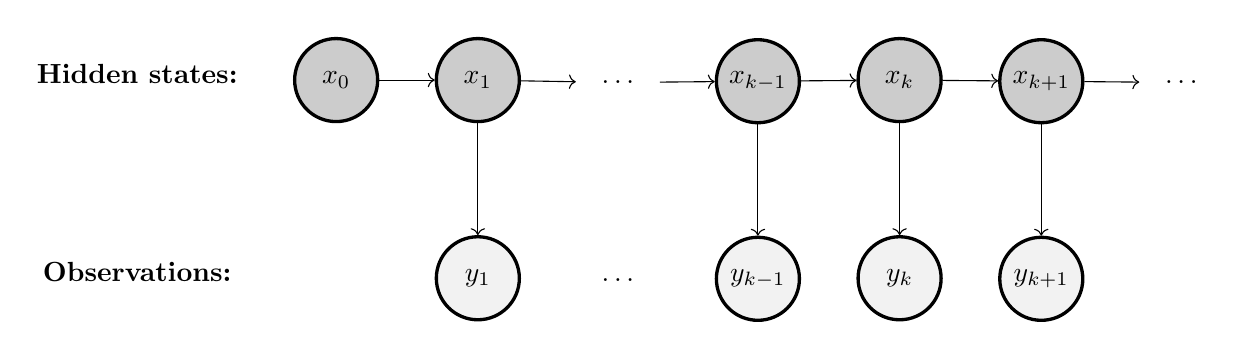
\begin{tikzpicture}
\tikzstyle{arrow} = [thick,->,stealth[length=15mm]]
\matrix[matrix of math nodes,column sep=2em,row
sep=4em,cells={nodes={circle,draw,minimum width=3em,inner sep=0pt}},
column 1/.style={nodes={rectangle, draw=none}},
column 4/.style={nodes={rectangle, draw=none}},
column 8/.style={nodes={rectangle,draw=none}},
row 1 column 2/.style={nodes={circle,fill=gray!40,draw=black,very thick}},
row 1 column 3/.style={nodes={circle,fill=gray!40,draw=black,very thick}},
row 1 column 5/.style={nodes={circle,fill=gray!40,draw=black,very thick}},
row 1 column 6/.style={nodes={circle,fill=gray!40,draw=black,very thick}},
row 1 column 7/.style={nodes={circle,fill=gray!40,draw=black,very thick}},
% row 1 column 9/.style={nodes={circle,fill=gray!40,draw=black,very thick}},
row 2 column 3/.style={nodes={circle,fill=gray!10,draw=black,very thick}},
row 2 column 5/.style={nodes={circle,fill=gray!10,draw=black,very thick}},
row 2 column 6/.style={nodes={circle,fill=gray!10,draw=black,very thick}},
row 2 column 7/.style={nodes={circle,fill=gray!10,draw=black,very thick}}] (m) {
\textbf{Hidden states:} &
  x_0 & x_1 & \ldots & x_{k-1} & x_k & x_{k+1} & \ldots  \\
\textbf{Observations:}
 & & y_1 & \ldots & y_{k-1} & y_k & y_{k+1}\\
};
\draw[->] (m-1-2) -- (m-1-3);
\draw[->] (m-1-3) -- (m-1-4);
\draw[->] (m-1-5) -- (m-1-6);
\draw[->] (m-1-6) -- (m-1-7);
\draw[->] (m-1-7) -- (m-1-8);
% \draw[->] (m-1-8) -- (m-1-9);
\draw[->] (m-1-3) -- (m-2-3);
\draw[->] (m-1-5) -- (m-2-5);
\draw[->] (m-1-6) -- (m-2-6);
\draw[->] (m-1-7) -- (m-2-7);
% \draw[->] (m-1-9) -- (m-2-9);
\draw[->] (m-1-4) -- (m-1-5);
\end{tikzpicture}

}
    \caption{Graphical illustration of the Markov property in a state-space model.}
    \label{fig:ssm-markov}
\end{figure}
This property allows us to express the joint probability distribution of the state sequence $x_{0:k}$ given the measurement sequence $y_{1:k}$ as follows:
\begin{equation} \label{eq:SSM-as-markov-example}
    \begin{split}
        p(x_{0:k} \mid y_{1:k}) \propto p(x_0) \prod_{i=1}^{k} p(x_{i} \mid x_{i-1})  \prod_{i=1}^{k} p(y_{i} \mid x_i)
    \end{split}
\end{equation}
 This is illustrated in Figure~\ref{fig:ssm-markov}. Next, we will review a discrete-time state-space model and discuss its components. 
%
\subsection{Discrete-time state-space models}
This thesis focuses on discrete-time probabilistic state-space models, characterized by the probability densities in Equation~\eqref{eq:ss-model}, followed by a description of their key components.
\begin{subequations}\label{eq:ss-model}
\begin{align}
    \begin{split} \label{eq:ssm-px0}
        x_0 &\sim p(x_0), 
    \end{split}\\
    \begin{split} \label{eq:ssm-transition}
        x_k \mid x_{k-1} &\sim p(x_k \mid x_{k-1}),
    \end{split}\\
    \begin{split} \label{eq:ssm-observation}
        y_k \mid x_k &\sim p(y_k \mid x_k),
    \end{split}
\end{align}
\end{subequations}
In the framework \eqref{eq:ss-model}, $k \in \mathbb{N}$ represents the discrete-time index. State variable $x_k \in \mathbb{R}^{n_x}$ represents the latent state at time $k$, which evolves over time according to a probabilistic dynamic model. Observation $y_k \in \mathbb{R}^{n_y}$ is the observed data at time $k$, which is related to the hidden state through a probabilistic observation model. 

The state transition model in Equation~\eqref{eq:ssm-transition}, describes how the state evolves from one time step to the next time step. The observation model in Equation~\eqref{eq:ssm-observation}, describes how the observed measurement depends on the underlying state. Initial state distribution $p(x_0)$ in Equation~\eqref{eq:ssm-px0}, specifying the uncertainty about the state at the beginning of the process. 
% Process noise represents the uncertainty in the state transition model, often modeled as random noise affecting the evolution of the state. Measurement noise accounts for the uncertainty in the observations and captures the deviation of the measurements from the true state.

Probabilistic state-space models inherently rely on the Markov property introduced in Definition \ref{def:markov-property}. The hidden states $x_k$ are assumed to form a Markov process. This property is essential for performing tasks such as filtering and prediction.

In this thesis, we consider two classes of discrete-time state-space models: the affine Gaussian model, described in Section~\ref{sec:affine-gaussian-model}, and the conditionally Gaussian model, covered in Section~\ref{sec:conditionally-gaussian-model}

\section{Statistical State Estimation}
The primary focus of this thesis is state estimation. In the previous section, we discussed how a probabilistic state-space model connects hidden states to noisy measurements. Statistical state estimation methods such as filtering and smoothing, enable the inference of these hidden states from noisy observations.

The key foundation of statistical state estimation is Bayes' rule, which provides a formal framework for updating beliefs about the states as new data is acquired. This rule is introduced in Theorem~\ref{th:Bayes-rule}.
%
\begin{theorem}[Bayes' rule] \label{th:Bayes-rule}
    Given the prior of $x$ as $p(x)$, and the conditional density $p(y \mid x)$, the probability density of $x$ given $y$ is 
    \begin{equation} \label{eq:bayes-theorem}
        p(x \mid y) = \frac{p(y \mid x) p(x)}{ p(y)} = \frac{p(y \mid x) p(x)}{\int p(y \mid x) p(x) dx}.
    \end{equation}
\end{theorem}
%
Bayes' rule enables the determination of filtering and smoothing densities, which are mathematically defined in Definitions~\ref{def:filtering} and \ref{def:smoothing}, respectively.
%
\begin{definition}[Filtering] \label{def:filtering}
    The objective of the Bayesian filtering problem is to determine the posterior distribution of the state $x$ at the current step $k$, given the observations up to time $k$, represented as $p(x_k \mid y_{1:k})$ for $k = \{1, \ldots, N\}$, where $N$ is the total number of time steps. It consists of the following equations~\citep[Theorem 6.5]{sarkka2023bayesian}:
    \begin{subequations}
    \begin{align}
        \begin{split} \label{eq:filter-prediction}
            p(x_k \mid y_{1:k-1}) & = \int p(x_k \mid x_{k-1}) p(x_{k-1} \mid y_{1:k-1}) dx_{k-1},
            \end{split}\\
            \begin{split} \label{eq:filter-update}
            p(x_k \mid y_{1:k}) &= \frac{p(y_k \mid x_k)p(x_k \mid y_{1:k-1})}{\int p(y_k \mid x_k)p(x_k \mid y_{1:k-1}) dx_k}.
        \end{split}
    \end{align}
    \end{subequations}
    The prediction step in Equation~\eqref{eq:filter-prediction} predicts the current state based on the previous state estimate and the state transition model through Chapman–Kolmogorov~\citep{[?]} equation.
    
    The update step in Equation~\eqref{eq:filter-update} involves refining the predicted density, $p(x_k \mid y_{1:k-1})$, by incorporating the new measurement $y_k$ and using the Bayes' rule presented in Theorem~\ref{th:Bayes-rule}.
\end{definition}
%
\begin{definition}[Smoothing] \label{def:smoothing}
    Given the filtering results, Bayesian smoother aims to compute the posterior distribution of the system states given all available data, including future observations, that is, $p(x_k \mid y_{1:N})$ for $k = \{1, \ldots, N\}$ as follows \citep[Theorem 12.1]{sarkka2023bayesian}:
    \begin{equation} \label{eq:filter-smoothing}
        \begin{split}
            &p(x_k \mid y_{1:N}) = p(x_k \mid y_{1:k}) \int \frac{p(x_{k+1} \mid x_k) p(x_{k+1} \mid y_{1:N})}{p(x_{k+1} \mid y_{1:N})} dx_{k+1}.
        \end{split}
    \end{equation}
    Given the distribution $p(x_N \mid y_{1:N})$ from the filtering solutions, the process described in Equation~\eqref{eq:filter-smoothing} involves performing a backward iteration for $k = \{N-1, \ldots, 1\}$.
\end{definition}
%
The filtering and smoothing equations are generally intractable for a state-space model of the form~\eqref{eq:ss-model}. However, in the special case of an affine state-space model with additive Gaussian noise, closed-form solutions exist, as described in Section~\ref{sec:affine-gaussian-model}. For nonlinear models with non-Gaussian noise, in this thesis, we will rely on approximations and use conditionally Gaussian models, which will be detailed in  Section~\ref{sec:conditionally-gaussian-model}. 

\section{State estimation in affine Gaussian models}\label{sec:affine-gaussian-model}
Discrete-time affine Gaussian models have the following form:
\begin{subequations} \label{eq:affine-gaussian-model}
    \begin{align}
        \begin{split} \label{eq:affine-gaussian-x0}
            x_0 &\sim \mathcal{N}(m_0, P_0), 
        \end{split}\\
        \begin{split} \label{eq:affine-gaussian-dynamic}
            x_k \mid x_{k - 1} &\sim \mathcal{N}(F_{k-1} x_{k-1} + c_{k-1} , Q_{k-1}), 
        \end{split}\\
        \begin{split} \label{eq:affine-gaussian-measurement}
            y_k \mid x_k &\sim \mathcal{N}(H_k x_k + d_k,  R_k),
        \end{split}
\end{align}
\end{subequations}
where $\mathcal{N}$ is a Gaussian distribution and $P_0$, $Q_{k-1}$, and $R_k$ are the covariance matrices of the initial state, transition noise, and measurement noise, respectively. The key feature of an affine SMM, as described in Equation~\eqref{eq:affine-gaussian-model}, is that the pairs of random variables $(x_k, x_{k - 1})$ in Equation~\eqref{eq:affine-gaussian-dynamic} and $(y_k, x_k)$ in Equation~\eqref{eq:affine-gaussian-measurement} are jointly Gaussian. This allows for closed-form solutions for posterior mean and covariance~\citep[subsection 1.4.14]{bar2004estimation}. Specifically, the Kalman filter~\citep{kalman1960new} provides a solution for filtering problems, while the Rauch–Tung–Striebel smoother~\citep{rauch1965maximum} addresses smoothing problems. In this section, we provide an overview of these two methods.
%
\paragraph{\textbf{Discrete-time recursive Kalman filter.}} The discrete-time recursive Kalman filter can be obtained as follows~\citep[Theorem 6.6]{sarkka2023bayesian}. Assume that we have the filtering distribution of the previous time step as $p(x_{k-1} \mid y_{1: k - 1}) = \mathcal{N}(m^f_{k-1}, P^f_{k-1})$. Then, in prediction step we need to find $p(x_{k} \mid y_{1, k}) \sim \mathcal{N}(m_{k}^-, P_{k}^-)$ as
    \begin{equation} \label{eq:affine-model-prediction}
        \begin{split}
            m_{k}^- &= F_{k-1} m^f_{k-1} + c_{k-1}, \\
            P_{k}^- &= F_{k-1} P^f_{k-1} F^\top_{k-1} + Q_{k-1}.
        \end{split}
    \end{equation}
In the Kalman filter's update step with measurement $y_{k}$, we need to determine $p(x_{k} \mid y_{1:k}) \sim \mathcal{N}( m^f_{k}, P^f_{k})$ which is parametrized as follows:
    \begin{equation} \label{eq:affine-model-update}
        \begin{split}
            S_k & = H_k P_{k}^- H_k^\top + R_k,\\
            K_k &=  P_{k}^- H_k^\top S_k^{-1},\\
            m^f_{k} &= m_{k}^- + K_k (y_{k} - H_k m^-_{k} - d_k ),\\
            P^f_{k} &= P_{k}^- - K_k S_k K_k^\top.
        \end{split}
    \end{equation}
The Kalman filter procedure is summarized in Algorithm~\ref{alg:KF}.
\begin{algorithm}[!htb]
    \caption{Kalman filter}\label{alg:KF}
    \begin{algorithmic}[1]
        \renewcommand{\algorithmicrequire}{\textbf{Input:}}
        \renewcommand{\algorithmicensure}{\textbf{Output:}}
        \REQUIRE Measurements $y_{1:N}$, initial distribution $x_0 \sim \mathcal{N}(x_0; m_0, P_0)$, transition model $x_k = \mathcal{N}(x_k; F_{k-1} x_{k-1} + c_{k-1} , Q_{k-1}$ and observation model $y_k =  \mathcal{N}(x_k; H_k x_k + d_k,  R_k)$.
        \ENSURE Filtering distributions $\big\{p(x_k \mid y_{1: k})  = \mathcal{N}(x_k; m^f_k, P^f_k)\big\}_{k = 0}^N$.
        \STATE{Set $m^f_0 = m_0$, and $P^f_0 = P_0$}
        \FOR{$k\gets 1$ \textbf{to} $N$}
        \STATE \COMMENT{Prediction step}
            \STATE {Set $m_{k}^- \gets F_{k-1} m^f_{k-1} + c_{k-1}$ and $P_{k}^- \gets F_{k-1} P^f_{k-1} F^\top_{k-1} + Q_{k-1}$}
            \STATE \COMMENT{Update step}
            \STATE  Set $
            K_k \gets  P_{k}^- H_k^\top (H_k P_{k}^- H_k^\top + R_k)^{-1}$
             \STATE Set $ m^f_{k} \gets m_{k}^- + K_k (y_{k} - H_k m^-_{k} - d_k ) $, and $P^f_{k} \gets P_{k}^- - K_k S_k K_k^\top$
        \ENDFOR
    \end{algorithmic}
\end{algorithm}
\paragraph{\textbf{Discrete-time recursive Rauch–Tung–Striebel smoother.}} After having the filtering distribution for all time steps and knowing that $p(x_N \mid y_{1:N}) = \mathcal{N}(m^s_N, P^s_N) = \mathcal{N}(m^f_N, P^f_N)$, the discrete-time Rauch–Tung–Striebel smoother is then a backwards recursion for the
parameters $m^s_k$ and $P^s_k$, which is given by \citep[Theorem 12.2]{sarkka2023bayesian}
\begin{equation} \label{eq:affine-model-smoother}
    \begin{split}
        G_k &= P^f_k F_k^\top [P^-_{k+1}]^{-1},\\
        m^s_k &= m^f_k + G_k (m^s_{k+1} - m^-_{k+1}),\\
        P^s_k &= P^f_k + G_k (P^s_{k+1} - P^-_{k+1})G_k^\top,
    \end{split}
\end{equation}
where $m^-_{k+1}$ and $P^-_{k+1}$  the predicted state and covariance for state $x_{k+1}$, which can be obtained using Equation~\eqref{eq:affine-model-prediction}. The RTS smoother procedure is summarized in Algorithm~\ref{alg:RTS-smoother}.
\begin{algorithm}[!htb]
    \caption{RTS smoother}\label{alg:RTS-smoother}
    \begin{algorithmic}[1]
        \renewcommand{\algorithmicrequire}{\textbf{Input:}}
        \renewcommand{\algorithmicensure}{\textbf{Output:}}
        \REQUIRE Filtering distributions $p(x_k \mid y_{1: k}) = \mathcal{N}(x_k; m^f_k, P^f_k)$, transition model $p(x_k \mid x_{k-1}) = \mathcal{N}(x_k; F_{k-1} x_{k-1} + c_{k-1} , Q_{k-1})$ for $k = \{1, \ldots, N\}$.
        \ENSURE Smoothing distributions $\big\{p(x_k \mid y_{1: N})  = \mathcal{N}(x_k; m^s_k, P^s_k)\big\}_{k=0}^N$.
        \STATE Set $m^s_N \gets m^f_N$, and $P^s_N \gets P^f_N$.
        \FOR{$k\gets N - 1$ \textbf{to} $0$}
            \STATE Set $G_k \gets P^f_k F_k^\top [F_{k} P^f_{k} F^\top_{k} + Q_{k}]^{-1}$\\[0.1cm]
            \STATE Set $m^s_k \gets m^f_k + G_k (m^s_{k+1} - F_{k} m^f_{k} - c_{k})$ \\[0.1cm]
            \STATE Set $P^s_k \gets P^f_k + G_k (P^s_{k+1} - F_{k} P^f_{k} F^\top_{k} - Q_{k})G_k^\top$
        \ENDFOR
    \end{algorithmic}
\end{algorithm}
%
\section{State estimation in conditionally Gaussian models} \label{sec:conditionally-gaussian-model}
Discrete-time conditionally Gaussian models consist of the following Gaussian distributions:
\begin{subequations} \label{eq:conditionally-gaussian-ssm}
    \begin{align}
        \begin{split} \label{eq:cond-gaussian-x0}
            x_0 &\sim \mathcal{N}(m_0, P_0),
        \end{split}\\
        \begin{split} \label{eq:cond-gaussian-dynamic}
            x_k \mid x_{k - 1} &\sim \mathcal{N}(\mathbb{E}[x_k \mid x_{k - 1}] , \mathbb{V}[x_k \mid x_{k-1}]), 
        \end{split}\\
        \begin{split} \label{eq:cond-gaussian-measurement}
            y_k \mid x_k &\sim \mathcal{N}(\mathbb{E}[y_k \mid x_k],  \mathbb{V}[y_k \mid x_k]).
        \end{split}
    \end{align}
\end{subequations}
Conditionally Gaussian models are a class of assumed density models in which the transition density, $p(x_k \mid x_{k-1})$, and the observation density, $p(y_k \mid x_k)$, belong to a specific class of distributions. In conditionally Gaussian models, both transition and observation densities are assumed to be Gaussian, characterized by their first two moments~\citep{maybeck1982stochastic, arasaratnam2009cubature, sarkka2008unscented} as in Equations~\eqref{eq:cond-gaussian-dynamic} and \eqref{eq:cond-gaussian-measurement}. In the following, we will present solutions for the assumed Gaussian filter and smoother. To do so, we first define the following terms for the conditional expected means and covariances in Equation~\eqref{eq:conditionally-gaussian-ssm}:
\begin{equation} \label{eq:con-gau-params}
    \begin{split}
        \mathcal{F}_k(x_{k-1}) &\coloneq \mathbb{E}[x_k \mid x_{k - 1}], \quad \mathcal{Q}_k(x_{k-1}) \coloneq \mathbb{V}[x_k \mid x_{k - 1}], \\
        \mathcal{H}_k(x_{k}) &\coloneq \mathbb{E}[y_k \mid x_{k}], \quad \mathcal{R}_k(x_{k}) \coloneq \mathbb{V}[y_k \mid x_{k}].
    \end{split}
\end{equation}
We also use the following Lemma:
\begin{lemma}
we consider the case where $x$ is composed of two random variables $x_1$ and $x_2$ then we have: $y=g(x_1,x_2)$ and the density $p(x) = p(x_1,x_2) = p(x_1 \mid x_2)p(x_2)$ then conditional mean and covariance are:
\begin{equation}
\begin{split}
    \mathbb{E}\{y\mid x_2\} &= \int g(x_1,x_2)p(x_1 \mid x_2)dx_1\\
    \mathbb{V}\{y\mid x_2\} &= \int (g(x_1,x_2) - \mathbb{E}\{g(x_1,x_2)\mid x_2\})(g(x_1,x_2) - \mathbb{E}\{g(x_1,x_2)\mid x_2\})^\top p(x_1 \mid x_2)dx_1
    \end{split}
\end{equation}
Then:
\begin{equation}
    \begin{split}
        \mathbb{E}\{y\} &= \int \int g(x_1,x_2)p(x_1,x_2)dx_2dx_1\\
        &= \int \int (g(x_1,x_2)p(x_1\mid x_2)dx_1)p(x_2)dx_2\\
        &=\mathbb{E}\{\mathbb{E}\{g(x_1,x_2)\mid x_2\}\}\\
        &=\mathbb{E}\{\mathbb{E}\{y\mid x_2\}\}
    \end{split}
\end{equation}
and:
\begin{equation}
    \begin{split}
     \mathbb{V}\{y\} &= \mathbb{E}\{yy^\top\} - \mathbb{E}\{y\}\mathbb{E}\{y\}^\top\\
     &= \mathbb{E}\{\mathbb{E}\{yy^\top \mid x_2\}\} - \mathbb{E}\{\mathbb{E}\{y\mid x_2\}\}\mathbb{E}\{\mathbb{E}\{y \mid x_2\}\}^\top\\
     &=\mathbb{E}\{\mathbb{V}\{y\mid x_2\}\} + \mathbb{E}\{\mathbb{E}\{y\mid x_2\}\mathbb{E}\{y\mid x_2\}^\top\}-\mathbb{E}\{\mathbb{E}\{y\mid x_2\}\}\mathbb{E}\{\mathbb{E}\{y\mid x_2 \}\}^\top\\
     &= \mathbb{E}\{\mathbb{V}\{y\mid x_2\}\}+\mathbb{V}\{\mathbb{E}\{y\mid x_2\}\}.
    \end{split}
\end{equation}
    \begin{equation}\label{eq:GSLR-moments}%
            \begin{split}
                \mathbb{E}[y] &=\mathbb{E}[\mathbb{E}[y\mid x]], \quad \mathbb{V}[y] = \mathbb{E}[\mathbb{V}[y\mid x]]+\mathbb{V}[\mathbb{E}[y\mid x]],\quad \mathbb{C}[y, x] =  \mathbb{C} [\mathbb{E}[y \mid x], x].
            \end{split}
        \end{equation}
\end{lemma}
\paragraph*{Gaussian assumed density filter} ...

prediction step
\begin{equation} \label{eq:assumed-Gaussian-prediction}
    \begin{split}
        m_k^- & = \mathbb{E}[x_k \mid y_{1: k-1}] \approx \mathbb{E}_{\pi}[\mathcal{F}_k(x_{k-1})],\\
         P_k^- &= \mathbb{V}_{\pi}[x_k \mid y_{1: k-1}] \approx \mathbb{V}_{\pi}[\mathcal{F}_k(x_{k-1})] + \mathbb{E}_{\pi}[\mathcal{Q}_k(x_{k-1}],
    \end{split}
\end{equation}
where the required moments are obtained based on $\pi \sim \mathcal{N}(x_{k-1}; m^f_{k-1}, P^f_{k-1})$.

Then, in the update step we have:
    \begin{equation} \label{eq:assumed-Gaussian-update}
        \begin{split}
            S_k & = \mathbb{V}_{\pi}[\mathcal{H}_k(x_{k})] + \mathbb{E}_{\pi}[\mathcal{R}_k(x_{k}],\\
            K_k &=  \mathbb{C}_{\pi}[x_k, \mathcal{H}_k(x_{k})] \, S_k^{-1},\\
            m^f_{k} &= m_{k}^- + K_k (y_{k} -  \mathbb{E}_{\pi}[\mathcal{H}_k(x_{k})]),\\
            P^f_{k} &= P_{k}^- - K_k S_k K_k^\top.
        \end{split}
    \end{equation}
The required moments in Equation~\eqref{eq:assumed-Gaussian-update} are obtained based with respect to $\pi \sim \mathcal{N}(x_{k}; m^-_{k}, P^-_{k})$.
\paragraph*{Gaussian assumed density smoother}...
\begin{equation} \label{eq:assumed-Gaussian-smoother}
    \begin{split}
        G_k &= \mathbb{C}_{\pi}[x_k, \mathcal{F}_{k+1}(x_{k+1})] [P^-_{k+1}]^{-1},\\
        m^s_k &= m^f_k + G_k (m^s_{k+1} - m^-_{k+1}),\\
        P^s_k &= P^f_k + G_k (P^s_{k+1} - P^-_{k+1})G_k^\top,
    \end{split}
\end{equation}
In Equation~\eqref{eq:assumed-Gaussian-smoother}, the required moment is obtained based on $\pi \sim \mathcal{N}(x_{k}; m^f_{k}, P^f_{k})$.

\textcolor{red}{explain sigma-point and first-order Taylor series}


\subsection{Example of state estimation in conditionally Gaussian model}
\textcolor{red}{An example of this model is stochastic volatility model.}
% Baye's rule + Conditional mean estimate + statistical linear regression + generalized statistical linear regression 
% \section{Nonlinear filtering and smoothing}
% \subsection{Affine models}
% \subsection{Non-affine models}

\chapter{Kalman smoothers from optimization viewpoint}
\label{ch:KS-optimization}
In this chapter, we approach the Kalman smoothing problem for a nonlinear state-space model with additive Gaussian noise from an optimization standpoint. We then explore both batch and recursive versions of the Gauss-Newton and Newton methods to solve the problem. The outcomes of Newton’s method are discussed in details in \citepub{eusipco}, with a focus on leveraging the problem's structure to develop a computationally efficient solution.
\section{Optimization problem}
 We are interested in solving state estimation problems in nonlinear SSMs with additive Gaussian noise of the form
\begin{subequations} \label{eq:nonlinear-additive-gaussian-ssm}
    \begin{align}
        \begin{split} \label{eq:cond-gaussian-x0}
            x_0 &\sim \mathcal{N}(x_0;\,  m_0, \, P_0),
        \end{split}\\
        \begin{split} \label{eq:cond-gaussian-dynamic}
            x_k \mid x_{k - 1} &\sim \mathcal{N}(x_k;\, f(x_{k-1}),\,  Q_{k-1}), 
        \end{split}\\
        \begin{split} \label{eq:cond-gaussian-measurement}
            y_k \mid x_k &\sim \mathcal{N}(y_k;\,  h(x_k), \, R_k).
        \end{split}
    \end{align}
\end{subequations}
This model is the specific type of conditionally Gaussian models where the parameters in Equation~\eqref{eq:con-gau-params} are
\begin{equation} \label{eq:nag-params}
    \begin{split}
        \mathcal{F}_k(x_{k-1}) &= f(x_{k-1}), \quad \mathcal{Q}_k(x_{k-1}) = Q_{k-1}, \\
        \mathcal{H}_k(x_{k}) &= h(x_k), \quad \mathcal{R}_k(x_{k}) = R_k.
    \end{split}
\end{equation}
The primary goal here is to determine the full smoothing distribution, $p(x_k \mid y_{1:N})$ for $k = \{1, \ldots, N\}$, when viewing the problem from an optimization perspective \citep{bell1994iterated, sarkka2020levenberg}. In this case, the idea is to find the maximum a posteriori (MAP) trajectory estimate, that is, the trajectory $x^*_{0:N}$ which maximizes the posterior distribution $p(x_{0:N} \mid y_{1:N})$ as follows:
\begin{equation} \label{eq:map-1}
    \begin{split}
        x^*_{0:N} = \argmax_{x_{0:N}}\big{\{}\, \, p(x_{0:N} \mid y_{1:N}) \propto p(x_0) \prod_{k=1}^{N} p(x_{k} \mid x_{k-1})  \prod_{k=1}^{N} p(y_{k} \mid x_k) \, \, \big{\}}.
    \end{split}
\end{equation}
Given the model of the form~\eqref{eq:nonlinear-additive-gaussian-ssm}, the distributions involved in Equation~\eqref{eq:map-1} are:
\begin{equation} \label{eq:gaussian-dist-nag}
    \begin{split}
        p(x_0) & \propto \exp{\bigg( -\frac{1}{2}\, (x_0 - m_0)^\top \, P_0^{-1} \, (x_0 - m_0) \bigg)}, \\
        p(x_{k} \mid x_{k-1}) & \propto \exp{\bigg( -\frac{1}{2}\, \big(x_{k} - f(x_{k-1})\big)^\top \, Q_{k-1}^{-1} \, \big(x_{k} - f(x_{k - 1})\big) \bigg)},\\
        p(y_{k} \mid x_k) & \propto \exp{\bigg( -\frac{1}{2}\, \big(y_{k} - h(x_{k})\big)^\top \, R_{k}^{-1} \, \big(y_{k} - h(x_{k})\big) \bigg)}.
    \end{split}
\end{equation}
By applying the distributions from Equation~\eqref{eq:gaussian-dist-nag} to Equation~\eqref{eq:map-1}, the MAP estimate in Equation~\eqref{eq:map-1} becomes equivalent to minimizing the following negative log-posterior:
\begin{equation} \label{eq:opt-L}
    x^*_{0:N} = \argmin_{x_{0:N}}{\, \, L(x_{0:N})},
\end{equation}
where the negative log-posterior is given by
\begin{equation} \label{eq:objective-function}
\begin{split}
    L(x_{0:N}) = \frac{1}{2} \lVert x_{0}
    - m_{0} \rVert^{2}_{P_{0}^{-1}} + \frac{1}{2} \sum_{k=1}^{N} \lVert x_{k} - f(x_{k-1}) \rVert^{2}_{Q_{k-1}^{-1}}  + \frac{1}{2} \sum_{k=1}^{N} \lVert y_{k} - h(x_{k}) \rVert^{2}_{R_{k}^{-1}}, 
    \end{split}
\end{equation}
where $\lVert x \rVert^{2}_{A} \coloneqq x^\top A x$. Taking an optimization perspective on the state estimation problem enables us to apply various optimization techniques \citep{wright1999numerical}. In the following sections, we will the batch Gauss-Newton and Newton methods, along with their recursive counterparts, which offer computationally efficient solutions.

\section{Batch Gauss-Newton method}
In this section, we begin by deriving the batch Gauss-Newton solution for the optimization problem in Equation~\eqref{eq:objective-function}. To achieve this, we first construct a canonical representation of the cost function in Equation~\eqref{eq:objective-function} \citep{bell1994iterated, sarkka2020levenberg} as follows:
\begin{equation} \label{eq:canonical-L}
    \begin{split}
        L(x_{0:N}) = \frac{1}{2} v^\top(x_{0:N}) \, A \, v(x_{0:N}), 
    \end{split}
\end{equation}
where 
\begin{equation} \label{eq:rx-A}
    \begin{split}
        v(x_{0:N}) = \begin{bmatrix}
            x_0 - m_0\\
            x_1 - f(x_0)\\
            y_1 - h(x_1)\\
            \vdots\\
            x_N - f(x_{N-1})\\
            y_N - h(x_N)
        \end{bmatrix}, \qquad A = \begin{bmatrix}
            P_0^{-1} & 0        & \ldots   & 0 & 0\\
            0        & Q_0^{-1} & \ldots   & 0 & 0\\
            0        & 0        & R_1^{-1} & \ldots & 0\\
            \vdots   & \vdots   & \vdots   & \vdots & \vdots\\
            0        & 0        & \ldots   & Q_{N-1}^{-1} & 0\\
            0        & 0        & \ldots   & 0 &  R_{N}^{-1}
        \end{bmatrix}
    \end{split}
\end{equation}
with $v(x_{0:N})\in \mathbb{R}^{(2N+1)n_x}$ and $A \in \mathbb{R}^{(2N+1)n_x \times (2N+1)n_x}$. With this representation, the optimization problem in Equation~\eqref{eq:opt-L} becomes a standard nonlinear least-squares problem, allowing us to apply the Gauss-Newton algorithm \citep[Chaps. 9 and 4 respectively]{bjorck1996numerical, boyd2004convex}. This is achieved by forming the first-order Taylor expansion of the nonlinear function $v(x)$ in the neighborhood of a nominal trajectory at $i$th iteration, $\hat{x}^{(i)}_{0:N}$, as follows:
\begin{equation} \label{eq:linear-rx}
    \begin{split}
        v(x_{0:N}) \approx v(\hat{x}^{(i)}_{0:N}) + V_x(\hat{x}^{(i)}_{0:N}) \, (x_{0:N} - \hat{x}^{(i)}_{0:N}),
    \end{split}
\end{equation}
where $V_x(.)$ is the Jacobian of the nonlinear function $v(x)$. Substituting this back into the nonlinear least-squares problem in Equation~\eqref{eq:canonical-L}, we obtain the following approximate Gauss-Newton cost function:
\begin{equation}
    \begin{split}
    L_{\text{GN}}^{(i)}(x_{0:N}) = \frac{1}{2} \lVert v(\hat{x}^{(i)}_{0:N}) + V_x(\hat{x}^{(i)}_{0:N}) (x_{0:N} - \hat{x}^{(i)}_{0:N}) \rVert^{2}_{A}.
    \end{split}
\end{equation}
Then in each iteration, the Gauss-Newton optimization problem is
\begin{equation} \label{eq:GN-opt}
    \hat{x}^{(i + 1)}_{0:N} = \argmin_{x_{0:N}}{\, \, L_{\text{GN}}^{(i)}(x_{0:N}) },
\end{equation}
with the batch solution as follows:
\begin{equation}
    \begin{split}
        \hat{x}^{(i + 1)}_{0:N} = \hat{x}^{(i)}_{0:N} +  \big(V_x^\top(\hat{x}^{(i)}_{0:N}) \, A \, V_x(\hat{x}^{(i)}_{0:N})\big)^{-1} \, V_x^\top(\hat{x}^{(i)}_{0:N}) \,  A \, (x_{0:N} - \hat{x}^{(i)}_{0:N}).
    \end{split}
\end{equation}
The Gauss-Newton method can also be seen as a variation of the Newton method with an approximated Hessian, a concept we will discuss further in Section~\ref{sec:batch-newton}.
\begin{remark}
    Computational complexity?
\end{remark}

\section{Recursive Gauss-Newton method}
For nonlinear SSM with additive Gaussian noise, in \citep{bell1994iterated}, it is proven that the GN-method is equivalent to the iterated extended Kalman smoother (IEKS), a recursive method with less computational complexity than batch GN-methods.

The IEKS solution proceeds by first obtaining the first order Taylor expansion of the nonlinear functions $f(.)$ and $h(.)$ in the SSM in Equation~\eqref{eq:nonlinear-additive-gaussian-ssm} around $\hat{x}^{(i)}_{k}$ and then then plug them back to the original SSM as:
\begin{equation} \label{eq:taylor-ssm}
    \begin{split}
        x_k \mid x_{k-1} &\sim \mathcal{N}(F_{k-1} x_{k-1} + c_{k-1}, Q_{k-1}),\\
        y_k \mid x_k &\sim \mathcal{N}(H_k x_k + d_k, R_k),
    \end{split}
\end{equation}
where 
\begin{align}
        F_{k-1} &= F_x(\hat{x}^{(i)}_{k - 1}), &&c_{k-1} = f(\hat{x}^{(i)}_{k - 1}) - F_x(\hat{x}^{(i)}_{k - 1}) \, \,  \hat{x}^{(i)}_{k - 1}, \\
        H_k &= H_x(\hat{x}^{(i)}_{k}),  && d_k = h(\hat{x}^{(i)}_{k }) - H_x(\hat{x}^{(i)}_{k}) \, \, \hat{x}^{(i)}_{k},
\end{align}
and $F_x(.)$ and $H_x(.)$ are the Jacobians of the nonlinear functions $f(.)$ and $h(.)$, respectively. Substituting Equation~\eqref{eq:taylor-ssm} in \eqref{eq:objective-function}, gives us the following approximated Gauss-Newton cost function 
\begin{equation} \label{eq:opt-affine}
    \begin{split}
        L^{(i)}_{GN}(x_{0:N}) =& \frac{1}{2} \lVert x_{0}
        - m_{0} \rVert^{2}_{P_{0}^{-1}} + \frac{1}{2} \sum_{k=1}^{N} \lVert x_{k}- F_{k-1} \, x_{k-1} - c_{k-1} \rVert^{2}_{Q_{k-1}^{-1}}  \\
        &+ \frac{1}{2} \sum_{k=1}^{N} \lVert y_{k}- H_{k} \, x_{k} - d_{k} \rVert^{2}_{R_{k}^{-1}}.
    \end{split}
\end{equation}
The solution to the optimization problem in Equation~\eqref{eq:opt-affine}, can be obtained efficiently using the the iterated extended Kalman smoother which is summarized in Algorithm~\ref{alg:IEKS}.
\begin{algorithm}[!htb]
    \caption{One iteration of iterated extended Kalman smoother (IEKS)}\label{alg:IEKS}
    \begin{algorithmic}[1]
        \renewcommand{\algorithmicrequire}{\textbf{Input:}}
        \renewcommand{\algorithmicensure}{\textbf{Output:}}
        \REQUIRE Measurements $y_{1:N}$, initial distribution $x_0 \sim \mathcal{N}(x_0; m_0, P_0)$, transition model $\trNonlinearAdditiveSSM$ and observation model $\obNonlinearAdditiveSSM$, initial guess for nominal trajectory $\hat{x}^{(i)}_{0:N}$.
        \ENSURE Approximated smoothed trajectory $\hat{x}^{(i + 1)}_{0:N}$ with distributions $\big\{p(x_k \mid y_{1: N})  = \mathcal{N}(x_k; m^s_k, P^s_k)\big\}_{k=0}^N$.
        \STATE Linearizing the transition and observation model around $\hat{x}^{(i)}_{0:N}$ and form the affine SMM as in Equation~\eqref{eq:taylor-ssm}
        \STATE Apply Kalman filter procedure in Algorithm~\ref{alg:KF} to find filtering distribution $\big\{p(x_k \mid y_{1: k})  = \mathcal{N}(x_k; m^f_k, P^f_k)\big\}_{k = 0}^N$
        \STATE Apply RTS smoother procedure in Algorithm~\ref{alg:RTS-smoother} to find smoothing distribution $\big\{p(x_k \mid y_{1: N})  = \mathcal{N}(x_k; m^s_k, P^s_k)\big\}_{k=0}^N$
        \STATE Set $\hat{x}^{(i + 1)}_{0:N} \gets \mathcal{N}(x_k; m^s_k, P^s_k)$
    \end{algorithmic}
\end{algorithm}
%
This method is extended in the iterated posterior linearization smoother (IPLS), which applies statistical linearization to create an affine approximation for nonlinear state-space models (SSMs) with additive Gaussian noise \citep{garcia2016iterated}. Additionally, this iterated approach is further generalized to accommodate more complex models, specifically nonlinear SSMs with nonadditive, non-Gaussian noise \citep{tronarp2018iterative}. 

\textcolor{red}{... Algorithms for IPLS and G-IPLS are needed here or in the previous chapter.}
\begin{remark}[Computational complexity]
    
\end{remark}
\begin{remark}
    Recently, S\"arkk\"a \& Svensson \citep{sarkka2020levenberg} developed line-search and Levenberg-Marquart extensions of the IEKS method.
\end{remark}
%%%
\section{Batch Newton method} \label{sec:batch-newton}
At every iteration $i$, Newton's method approximates a twice differentiable objective $L(x_{0:N})$ in Equation~\eqref{eq:objective-function} up to the second order in the neighborhood of a nominal trajectory $\hat{x}^{(i)}_{0:N}$ as follows \citep{wright1999numerical}:
\begin{equation} \label{eq:quadratic-approximation} 
\begin{split}
    L(x_{0:N}) \approx \,
    & L(\hat{x}^{(i)}_{0:N}) + \nabla L^\top(\hat{x}^{(i)}_{0:N}) \, \,(x_{0:N} - \hat{x}^{(i)}_{0:N})  \\
    &+ \frac{1}{2}(x_{0:N} - \hat{x}^{(i)}_{0:N})^\top \, \,  \nabla^{2}L(\hat{x}^{(i)}_{0:N}) \, \, (x_{0:N} - \hat{x}^{(i)}_{0:N}),
    \end{split}
\end{equation}
where $\nabla L(.)$ and $\nabla^{2}L(.)$ denote the gradient and the Hessian of $L(.)$, respectively. Using this quadratic approximation, we get the Newton update rule \citep{wright1999numerical}
\begin{equation} \label{eq:Newton-update}
    \hat{x}^{(i+1)}_{0:N} = \hat{x}^{(i)}_{0:N} - (\nabla^{2}L(\hat{x}^{(i)}_{0:N}))^{-1} \, \nabla L(\hat{x}^{(i)}_{0:N}).
\end{equation}
Connection to the Gauss-Newton method. 

Computational complexity of the solution
\section{Recursive Newton method}
Constructing the modified state-space model requires analyzing the first- and second-order approximations of the individual terms in Equation~\eqref{eq:objective-function}. Let use define transition dynamics terms of the objective function as
\begin{equation} \label{eq:opt-S}
    S(x_{0:N}) \coloneqq \sum_{k=1}^{N} S_{k}(x_{k}, x_{k-1}) = \sum_{k=1}^{N} \lVert x_{k} - f(x_{k-1}) \rVert^{2}_{Q_{k-1}^{-1}},
\end{equation}
Now, if we expand Equation~\eqref{eq:opt-S} around the current nominal trajectory $\hat{x}^{(i)}_{0:N}$ using the second-order Taylor approximation and do some basic algebraic manipulation, we arrive at the following decomposition of the quadratic expansion 
\begin{equation} \label{eq:modified_transition}
    \begin{split}
    S(x_{0:N}) \approx
        & \sum_{k=1}^{N} \lVert x_{k} - F_{k-1} \, x_{k-1} - c_{k-1} \rVert^{2}_{Q_{k-1}^{-1}} + \sum_{k=1}^{N} \lVert \hat{x}^{(i)}_{k-1} - x_{k-1} \rVert^{2}_{\Psi_{k-1}},
    \end{split}
\end{equation}
where
\begin{equation} \label{eq:approx-params-S}
    \begin{split}
        F_{k-1} &= F_{x}(\hat{x}^{(i)}_{k - 1}), \quad c_{k-1} = f(\hat{x}^{(i)}_{k - 1}) - F_x(\hat{x}^{(i)}_{k - 1}) \, \,  \hat{x}^{(i)}_{k - 1}, \\
        \Psi_{k-1} &= - F^{\top}_{x x}(\hat{x}^{(i)}_{k - 1}) \cdot Q_{k-1}^{-1} (\hat{x}^{(i)}_k - f(\hat{x}^{(i)}_{k - 1})).
    \end{split}
\end{equation}
In Equation~\eqref{eq:approx-params-S}, $F_{x x}(.)$ is a third-rank Hessian tensor of the transition function $f(.)$. The notation $(M \cdot v)$ refers to a tensor dot product so that $(M \cdot v)_{ij} = \sum_{k} M_{ijk} v_{k}$.
A similar second-order expansion can be carried out for the observation model term in Equation~\eqref{eq:objective-function}. Again, for convenience, we define the following
\begin{equation} \label{eq:opt-G}
    G(x_{0:N}) \coloneqq \sum_{k=1}^{N} G_{k}(x_{k}) = \sum_{k=1}^{N} \lVert y_{k} - h(x_{k}) \rVert^{2}_{R_k^{-1}},
\end{equation}
Similarly, by rearranging these terms, we can construct a specific decomposition of the quadratic expansion in Equation~\eqref{eq:opt-G}
\begin{equation} \label{eq:modified_observation}
    G(x_{0:N}) \! \approx \sum_{k=1}^{N} \lVert y_{k} - H_{k} \, x_{k} - d_{k} \rVert^{2}_{R_k^{-1}} + \! \sum_{k=1}^{N} \lVert \hat{x}^{(i)}_{k} - x_{k} \rVert^{2}_{\Gamma_{k}},
\end{equation}
where
\begin{equation} \label{eq:approx-params-G}
    \begin{split}
        H_{k} &= H_{x}(\hat{x}^{(i)}_{k}), \quad d_k = h(\hat{x}^{(i)}_{k}) - H_x(\hat{x}^{(i)}_{k}) \, \, \hat{x}^{(i)}_{k}, \\
        \Gamma_{k} &= - H_{x x}^{\top}(\hat{x}^{(i)}_{k}) \cdot R^{-1} (y_{k} - h(\hat{x}^{(i)}_{k})).
    \end{split}
\end{equation}
We can now take the second-order terms of the transition and observation functions in Equations~\eqref{eq:modified_transition} and \eqref{eq:modified_observation} and plug them back into the objective in Equation~\eqref{eq:objective-function} which leads to the following approximate Newton cost function 
\begin{align} 
    \label{eq:approx-objective-function}
    & L_{\text{N}}(x_{0:N}) = \,
    \frac{1}{2} \lVert x_{0} - m_{0} \rVert^{2}_{{P}_{0}^{-1}} + \frac{1}{2} \lVert x_{0} - \hat{x}_{0} \rVert^{2}_{{\Phi}_{0}^{-1}} \notag \\
    & \qquad + \frac{1}{2} \sum_{k=1}^{N} \lVert \hat{x}_{k} - x_{k} \rVert^{2}_{\Phi_{k}^{-1}}
    + \frac{1}{2} \sum_{k=1}^{N} \lVert y_{k} - H_{k} \, x_{k} - d_{k} \rVert^{2}_{R_{k}^{-1}} \notag \\
    & \qquad + \frac{1}{2} \sum_{k=1}^{N} \lVert x_{k}- F_{k-1} \, x_{k-1} - c_{k-1} \rVert^{2}_{Q_{k-1}^{-1}},
\end{align}
where 
\begin{equation}
    \begin{split}
        \Phi_{0} = \mathbf{\Psi}_{0}^{-1}, \quad \Phi_{k} = (\Psi_{k} + \Gamma_{k})^{-1}, \quad \Phi_{N} = \Gamma_{N}^{-1}.
    \end{split}
\end{equation}
The result in Equation~\eqref{eq:approx-objective-function} indicates that the second-order approximation of $L(.)$ can be viewed as a first-order approximation of the functions $f$ and $h$, augmented by an affine pseudo observation model, in which the expansion point $\hat{x}_{k}$ acts as a pseudo measurement of the state $x_{k}^{(i)}$. This interpretation of \eqref{eq:approx-objective-function} corresponds to the \emph{modified} state-space model of the form \citepub{eusipco}
\begin{align*}
    x_{k} & \approx F_{k-1} \, x_{k-1} + c_{k-1} + q_{k},&&  \, q_{k} \sim \mathcal{N}(0, Q), \\
    y_{k} & \approx H_{k} \, x_{k} + d_{k} + r_{k},&&  \, r_{k} \sim \mathcal{N}(0, R), \\
    \hat{x}_{k}^{(i)} & \approx x_{k} + e_{k},&& \, e_{k} \sim \mathcal{N}(0, \Phi_{k}),
\end{align*}
with a \emph{modified} prior distribution $x_{0} \sim \mathcal{N}(\tau_{0}, \Omega_{0})$
\begin{equation}
    \Omega_{0} = (P^{-1}_{0} + \Phi^{-1}_{0})^{-1}, \quad \tau_{0} = (P^{-1}_{0} + \Phi^{-1}_{0})^{-1} \, (P^{-1}_{0} m_0 + \Phi^{-1}_{0} \hat{x}_0).
\end{equation}
%
\chapter{Parallel-in-time state estimation}
\label{ch:parallel-fs}
This chapter is about "Parallelization of Bayesian filtering and smoothing + Parallel linearization and sigma point approximations + robustness (square-root methods + parallel) + parallel integrated measurement"

\section{The need for parallelism}
\citep{plancher2022gpu}
\begin{itemize}
    \item How to take advantage of the strengths of hardware
    \item 
\end{itemize}
\section{Parallel-scan algorithm} \label{sec:parallel-scan}
    The parallel-scan algorithm \citep{blelloch1989scans} offers an efficient approach to performing the all-prefix-sum operation. This operation involves computing cumulative results for a set of elements $\{a_k\}_{1 \leq k \leq N}$ using a binary associative operator $\Motimes$. Specifically, it generates the sequence:
    \begin{equation}
        [(a_1), \, (a_1 \Motimes a_2), \,\ldots, \, (a_1 \Motimes a_2 \Motimes \ldots \Motimes a_n)].
    \end{equation}
    
    While a direct sequential approach would require $O(N)$ time, the parallel-scan algorithm leverages the associative nature of $\Motimes$ to break the task into smaller, concurrent sub-tasks. This parallelism reduces the computation time to $O(\log(N))$, making the algorithm highly efficient for large-scale data processing. By enabling multiple segments to be processed independently and then merged, the algorithm significantly speeds up the all-prefix-sum operation. This algorithm is especially well-suited for GPUs as they can handle a large number of very small tasks across thousands of threads. 

    \textcolor{red}{The pseudocode for the parallel-scan algorithm is outlined in Algorithm... (explain the in-place transformation) Following this, we will explore an example of this method.}

    \paragraph{\textbf{Example.}} Let us assume we have the associative operator $\Motimes$, represented here as ordinary summation and denoted by $\Moplus$. Also, assume we have $N = 8$ numbers, $(a_i)|_{i = 1}^8$, given as follows:
    \begin{figure}[H]
        \centering
        \resizebox{\columnwidth}{!}{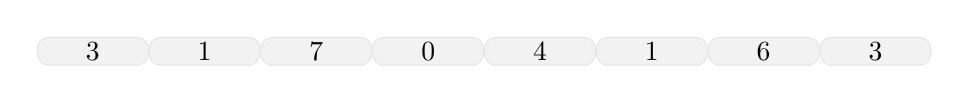
\begin{tikzpicture}
    \matrix[matrix of math nodes,column sep=0em,row
    sep=4em,cells={nodes={rectangle,draw=gray!20,  fill=gray!10,minimum width=1em,  minimum height=1em, text width=4em, align=center, rounded corners, inner sep=0pt}}] (m) {
       3 & 1 & 7 & 0 & 4 & 1 & 6 & 3 \\};
\end{tikzpicture}

}
    \end{figure}
    The objective is to compute the prefix-sums, also known as cumulative sum sequentially, on a CPU and in parallel on a GPU, while analyzing the algorithm's efficiency in terms of two components: work and span. The work represents the total number of operations performed, while the span is the length of the longest sequence of operations that cannot be parallelized.
    \paragraph{\textbf{Prefix-sums on a simple CPU.}} 
    The prefix-sums in a CPU can be obtained using a simple for-loop where we need exactly $N$ adds operations. The output will be as follows: 
    \begin{figure}[H]
        \centering
        \resizebox{\columnwidth}{!}{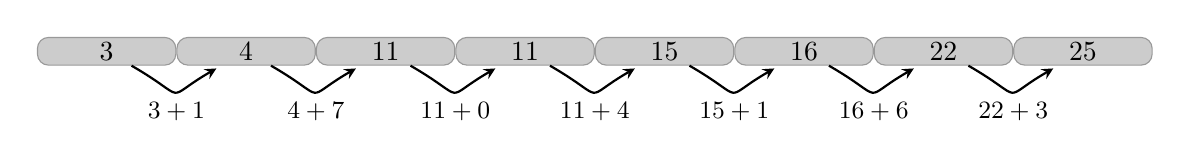
\begin{tikzpicture}[>=stealth,->,shorten >=2pt,looseness=2,auto]
    \matrix[matrix of math nodes,column sep=0em,row
    sep=4em,cells={nodes={rectangle,draw=gray!80,  fill=gray!40,minimum width=1em,  minimum height=1em, text width=5em, align=center, rounded corners, inner sep=0pt}}] (m) {
      |(a_1)| 3 & |(a_2)| 4 & |(a_3)| 11 & |(a_4)| 11 & |(a_5)| 15 & |(a_6)| 16 & |(a_7)| 22 & |(a_8)| 25 \\};
      \begin{scope}[every node/.style={font=\small\itshape}]
          \draw[thick] (a_1) to [bend right] node [below] {$3 + 1$} (a_2);
          \draw[thick] (a_2) to [bend right] node [below] {$4 + 7$} (a_3);
          \draw[thick] (a_3) to [bend right] node [below] {$11 + 0$} (a_4);
          \draw[thick] (a_4) to [bend right] node [below] {$11 + 4$} (a_5);
          \draw[thick] (a_5) to [bend right] node [below] {$15 + 1$} (a_6);
          \draw[thick] (a_6) to [bend right] node [below] {$16 + 6$} (a_7);
          \draw[thick] (a_7) to [bend right] node [below] {$22 + 3$} (a_8);
      \end{scope}
\end{tikzpicture}}
    \end{figure}
    This sequential algorithm has both work and span of $O(N)$.
    \paragraph{\textbf{Prefix-sums on a GPU.}} To compute the prefix-sums in parallel, one approach is to use the parallel-scan algorithm \citep{blelloch1989scans}, which operates in two phases: up-sweep and down-sweep, requiring $2\, \log\,(N)$ steps in total. In this example, the up-sweep phase requires $\log\,(8) = 3$ steps, as follows:
    \begin{figure}[H]
        \centering
        \resizebox{\columnwidth}{!}{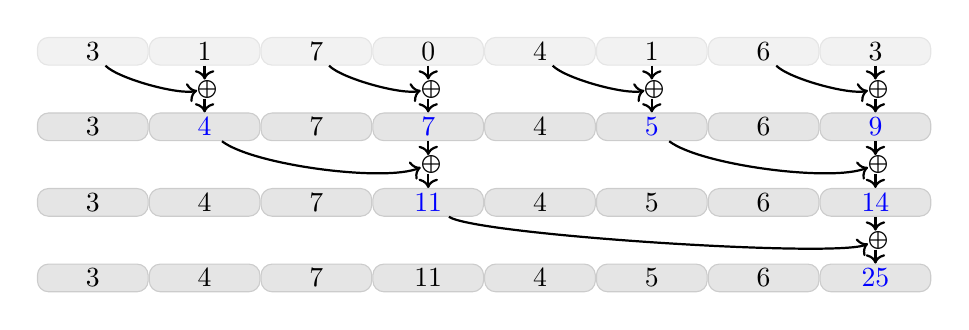
\begin{tikzpicture}
    \matrix[matrix of math nodes,column sep=0em,row
    sep=0.5em,
    row 1/.style={nodes={rectangle,draw=gray!20,fill=gray!10,minimum width=1em,  minimum height=1em, text width=4em, align=center, rounded corners, inner sep=0pt}},
    row 2/.style={nodes={rectangle,draw=white,minimum width=0.5em,  minimum height=0.5em, text width=0.5em, align=center, rounded corners, inner sep=0pt}},
    row 3/.style={nodes={rectangle,draw=gray!40,fill=gray!20,minimum width=1em,  minimum height=1em, text width=4em, align=center, rounded corners, inner sep=0pt}},
    row 4/.style={nodes={rectangle,draw=white,minimum width=0.5em,  minimum height=0.5em, text width=0.5em, align=center, rounded corners, inner sep=0pt}},
    row 5/.style={nodes={rectangle,draw=gray!40,fill=gray!20,minimum width=1em,  minimum height=1em, text width=4em, align=center, rounded corners, inner sep=0pt}},
    row 6/.style={nodes={rectangle,draw=white,minimum width=0.5em,  minimum height=0.5em, text width=0.5em, align=center, rounded corners, inner sep=0pt}},
    row 7/.style={nodes={rectangle,draw=gray!40,fill=gray!20,minimum width=1em,  minimum height=1em, text width=4em, align=center, rounded corners, inner sep=0pt}}] (m) {
      |(a_1)| 3 & |(a_2)| 1 & |(a_3)| 7 & |(a_4)| 0 & |(a_5)| 4 & |(a_6)| 1 & |(a_7)| 6 & |(a_8)| 3 \\
      %
      & |(b_2)| \Moplus &  & |(b_4)| \Moplus &  & |(b_6)| \Moplus &  & |(b_8)| \Moplus\\
      %
      |(c_1)| 3 & |(c_2)| \textcolor{blue}{4} & |(c_3)| 7 & |(c_4)| \textcolor{blue}{7} & |(c_5)| 4 & |(c_6)| \textcolor{blue}{5} & |(c_7)| 6 & |(c_8)| \textcolor{blue}{9} \\
       %
        &  &  & |(d_4)| \Moplus &  &  &  & |(d_8)| \Moplus\\
        %
        |(e_1)| 3 & |(e_2)| 4 & |(e_3)| 7 & |(e_4)| \textcolor{blue}{11} & |(e_5)| 4 & |(e_6)| 5 & |(e_7)| 6 & |(e_8)| \textcolor{blue}{14} \\
        %
        &  &  &  &  &  &  & |(f_8)| \Moplus\\
        %
        |(g_1)| 3 & |(g_2)| 4 & |(g_3)| 7 & |(g_4)| 11 & |(g_5)| 4 & |(g_6)| 5 & |(g_7)| 6 & |(g_8)| \textcolor{blue}{25} \\
        };
       %
      \begin{scope}[every node/.style={font=\small\itshape}]
          \draw[->, thick] (a_1) to [bend right, looseness=0.5] (b_2);
          \draw[->, thick] (a_2) -- (b_2);
          \draw[->, thick] (a_3) to [bend right, looseness=0.5] (b_4);
          \draw[->, thick] (a_4) -- (b_4);
          \draw[->, thick] (a_5) to [bend right, looseness=0.5] (b_6);
          \draw[->, thick] (a_6) -- (b_6);
          \draw[->, thick] (a_7) to [bend right, looseness=0.5] (b_8);
          \draw[->, thick] (a_8) -- (b_8);
          \draw[->, thick] (b_2) -- (c_2);
          \draw[->, thick] (b_4) -- (c_4);
          \draw[->, thick] (b_6) -- (c_6);
          \draw[->, thick] (b_8) -- (c_8);
          \draw[->, thick] (c_2) to [bend right, looseness=0.5] (d_4);
          \draw[->, thick] (c_4) -- (d_4);
          \draw[->, thick] (c_6) to [bend right, looseness=0.5] (d_8);
          \draw[->, thick] (c_8) -- (d_8);
          \draw[->, thick] (d_4) -- (e_4);
          \draw[->, thick] (d_8) -- (e_8);
          \draw[->, thick] (e_4) to [bend right, looseness=0.2] (f_8);
          \draw[->, thick] (e_8) -- (f_8);
          \draw[->, thick] (f_8) -- (g_8);
      \end{scope}
\end{tikzpicture}
}
    \end{figure}
    The down-sweep phase also requires $\log\,(8) = 3$ steps, as follows:
    \begin{figure}[H]
        \centering
        \resizebox{\columnwidth}{!}{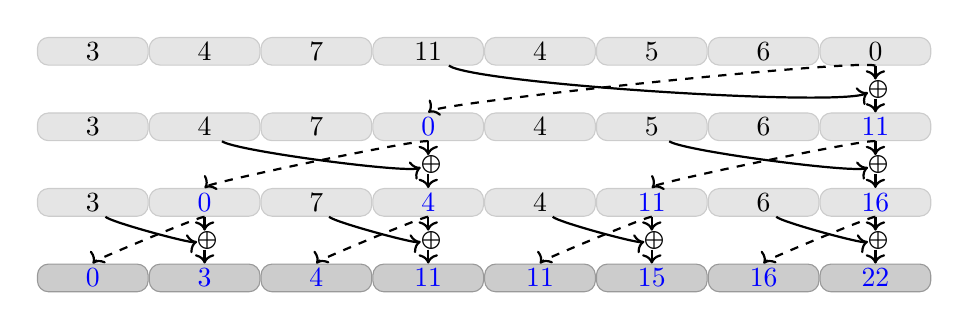
\begin{tikzpicture}
    \matrix[matrix of math nodes,column sep=0em,row
    sep=0.5em,
    row 1/.style={nodes={rectangle,draw=gray!40,fill=gray!20,minimum width=1em,  minimum height=1em, text width=4em, align=center, rounded corners, inner sep=0pt}},
    row 2/.style={nodes={rectangle,draw=white,minimum width=0.5em,  minimum height=0.5em, text width=0.5em, align=center, rounded corners, inner sep=0pt}},
    row 3/.style={nodes={rectangle,draw=gray!40,fill=gray!20,minimum width=1em,  minimum height=1em, text width=4em, align=center, rounded corners, inner sep=0pt}},
    row 4/.style={nodes={rectangle,draw=white,minimum width=0.5em,  minimum height=0.5em, text width=0.5em, align=center, rounded corners, inner sep=0pt}},
    row 5/.style={nodes={rectangle,draw=gray!40,fill=gray!20,minimum width=1em,  minimum height=1em, text width=4em, align=center, rounded corners, inner sep=0pt}},
    row 6/.style={nodes={rectangle,draw=white,minimum width=0.5em,  minimum height=0.5em, text width=0.5em, align=center, rounded corners, inner sep=0pt}},
    row 7/.style={nodes={rectangle,draw=gray!80,fill=gray!40,minimum width=1em,  minimum height=1em, text width=4em, align=center, rounded corners, inner sep=0pt}}] (m) {
      |(a_1)| 3 & |(a_2)| 4 & |(a_3)| 7 & |(a_4)| 11 & |(a_5)| 4 & |(a_6)| 5 & |(a_7)| 6 & |(a_8)| 0 \\
      %
      &  &  &  &  &  &  & |(b_8)| \Moplus\\
      %
      |(c_1)| 3 & |(c_2)| 4 & |(c_3)| 7 & |(c_4)| \textcolor{blue}{0} & |(c_5)| 4 & |(c_6)| 5 & |(c_7)| 6 & |(c_8)| \textcolor{blue}{11} \\
       %
        &  &  & |(d_4)| \Moplus &  &  &  & |(d_8)| \Moplus\\
        %
        |(e_1)| 3 & |(e_2)| \textcolor{blue}{0} & |(e_3)| 7 & |(e_4)| \textcolor{blue}{4} & |(e_5)| 4 & |(e_6)| \textcolor{blue}{11} & |(e_7)| 6 & |(e_8)| \textcolor{blue}{16} \\
        %
        & |(f_2)| \Moplus &  &  |(f_4)| \Moplus&  &  |(f_6)| \Moplus&  & |(f_8)| \Moplus\\
        %
        |(g_1)| \textcolor{blue}{0} & |(g_2)| \textcolor{blue}{3} & |(g_3)| \textcolor{blue}{4} & |(g_4)| \textcolor{blue}{11} & |(g_5)| \textcolor{blue}{11} & |(g_6)| \textcolor{blue}{15} & |(g_7)| \textcolor{blue}{16} & |(g_8)| \textcolor{blue}{22} \\
        };
       %
      \begin{scope}[every node/.style={font=\small\itshape}]
          \draw[->, thick] (a_4) to [bend right, looseness=0.2] (b_8);
          \draw[->, thick] (a_8) to (b_8);
          \draw[->, thick] (b_8) to (c_8);
          \draw[->, thick, dashed] (a_8.south) to [bend right, looseness=0.1] (c_4.north);
          %
          \draw[->, thick] (c_2) to [bend right, looseness=0.2] (d_4);
          \draw[->, thick] (c_4) to (d_4);
          \draw[->, thick] (d_4) to (e_4);
          \draw[->, thick, dashed] (c_4.south) to [bend right, looseness=0.1] (e_2.north);
          %
          \draw[->, thick] (c_6) to [bend right, looseness=0.2] (d_8);
          \draw[->, thick] (c_8) to (d_8);
          \draw[->, thick] (d_8) to (e_8);
          \draw[->, thick, dashed] (c_8.south) to [bend right, looseness=0.1] (e_6.north);
          %
          \draw[->, thick] (e_1) to [bend right, looseness=0.2] (f_2);
          \draw[->, thick] (e_2) to (f_2);
          \draw[->, thick] (f_2) to (g_2);
          \draw[->, thick, dashed] (e_2.south) to [bend right, looseness=0.1] (g_1.north);
          %
          \draw[->, thick] (e_3) to [bend right, looseness=0.2] (f_4);
          \draw[->, thick] (e_4) to (f_4);
          \draw[->, thick] (f_4) to (g_4);
          \draw[->, thick, dashed] (e_4.south) to [bend right, looseness=0.1] (g_3.north);
          %
          \draw[->, thick] (e_5) to [bend right, looseness=0.2] (f_6);
          \draw[->, thick] (e_6) to (f_6);
          \draw[->, thick] (f_6) to (g_6);
          \draw[->, thick, dashed] (e_6.south) to [bend right, looseness=0.1] (g_5.north);
          %
          \draw[->, thick] (e_7) to [bend right, looseness=0.2] (f_8);
          \draw[->, thick] (e_8) to (f_8);
          \draw[->, thick] (f_8) to (g_8);
          \draw[->, thick, dashed] (e_8.south) to [bend right, looseness=0.1] (g_7.north);
      \end{scope}
\end{tikzpicture}
}
    \end{figure}
    In addition to Blelloch's parallel-scan algorithm, several other algorithms can be used to compute prefix sums. For a review of these methods, see \citep{pibiri2021practical}. We will revisit this algorithm in the following sections.
    
\section{Parallel state estimation in state-space model}
The parallel-scan framework outlined in Section~\ref{sec:parallel-scan} has recently been employed to create parallel formulations of Bayesian filtering and smoothing \cite{sarkka2020temporal}. This approach achieves the same results as the sequential Bayesian filtering presented in Equation~\eqref{eq:filter-update} and smoothing in Equation~\eqref{eq:filter-smoothing}, but with logarithmic time complexity.
    \subsection{Parallel Bayesian filter}
        To establish parallel formulations of the Bayesian filter, it is necessary to define an appropriate element $a_k$ and the binary associative operator $\Motimes$. It has been shown in \cite[Definition 2 and Theorem 3]{sarkka2020temporal} that, given two positive functions $g_i(y)$ and $g_j(y)$, along with two conditional densities $f_i(x \mid y)$ and $f_j(x \mid y)$, selecting $a_k = (f_k, g_k)$ as
        \begin{equation}  \label{eq:gen-filter-init}
            \begin{split}
                f_k(x_k \mid x_{k-1}) &= p(x_k \mid y_k, x_{k-1}), \\
                g_k(x_{k-1}) &= p(y_k \mid x_{k-1}),
            \end{split}
        \end{equation}
        where $p(x_1 \mid y_1,x_0) = p(x_1 \mid y_1)$ and $p(y_1 \mid x_0)= p(y_1)$, and defining the associative binary operator $(f_i,g_i) \, \Motimes \, (f_j,g_j) \coloneqq (f_{ij},\, g_{ij})$ as
        \begin{equation} \label{eq:gen-filter-op}
            \begin{split}
                f_{ij}(x \mid z) &= \frac{\int{g_j(y)f_j(x \mid y)}f_i(y\mid z)dy}{\int{g_j(y)}f_i(y \mid z)dy},\\
                g_{ij}(z) &= g_i(z)\int{g_j(y)f_i(y \mid z)dy},
            \end{split}
        \end{equation}
         The results of the $k$th prefix sum of the elements $a_k$ under $\Motimes$ recover the filtering distribution at step $k$ as well as the marginal likelihood of the observations, that is,
        \begin{equation}
        a_1\Motimes \dots \Motimes a_k = \binom{p(x_k \mid y_{1:k})}{p(y_{1:k})}.
        \label{eq:gen-filter-res}
        \end{equation}
        \paragraph{\textbf{Parallel linear Gaussian filter.}} In the specific case of an affine Gaussian state-space model, as given in Equation~\eqref{eq:affine-gaussian-model}, closed-form expressions for the element $a_k$ in Equation~\eqref{eq:gen-filter-init}, and the binary associative operator $\Motimes$ in Equation~\eqref{eq:gen-filter-op} have been derived. In this case, the element $a_k$ is specified by the following parameters:
        \begin{equation} \label{eq:linear-filter-init}
            \begin{split}
               f_k(x_k \mid x_{k-1}) &= p(x_k \mid  y_k, x_{k-1}) =\mathcal{N}(x_k; A_k x_{k-1} + b_k, C_k),\\
               g_k(x_{k-1}) &= p(y_k \mid x_{k-1})\propto \mathcal{N}_I(x_{k-1}; \eta_k,J_k)
            \end{split}
        \end{equation}
        where $\mathcal{N}_I$ is the information form of the Gaussian distribution. Applying standard Gaussian algebra, the parameters in Equation~\eqref{eq:linear-filter-init} are derived as follows:
        \begin{equation} \label{eq:parallel-parameters-filtering}
            \begin{split}
                A_k &= (I_{n_x} - K_k H_k)F_{k-1}, \\
                b_k &= c_{k-1} + K_k( y_k - H_k c_{k-1} - d_{k-1}), \\
                C_k & = (I_{n_x} -K_k H_k) Q_{k-1}, \\
                J_k &= (H_k F_{k-1})^\top S_k^{-1} H_k F_{k-1} \\
                \eta_k &= (H_k F_{k-1} )^\top S_k^{-1} H_k  (y_k - H_k c_{k-1} - d_k).
            \end{split}
        \end{equation}
        where $ K_k = Q_{k-1}{H_k}^\top S_k^{-1}$, and $
        S_k = H_k Q_{k-1} H_k^\top+ R_k$. Furthermore, given $a_i$ and $a_j$ with the specified parameters in Equation~\eqref{eq:parallel-parameters-filtering}, the binary associative operator $a_i \Motimes a_j = a_{ij}$ can be computed using the following parameterization \cite[lemma 8]{sarkka2020temporal}:
        \begin{equation} \label{eq:op-filter}
            \begin{split}
                A_{ij} &= A_j (I_{n_x} + C_i J_j)^{-1} A_i,\\
                b_{ij} &= A_j (I_{n_x} + C_i J_j)^{-1} (b_i + C_i \eta_j) + b_j,\\
                C_{ij} &= A_j (I_{n_x} + C_i J_j)^{-1} C_i A_j^\top + C_j,\\
                \eta_{ij} &= A_i^\top (I_{n_x} + J_j C_i)^{-1} (\eta_j - J_j b_i) + \eta_i,\\
                J_{ij} &= A_i^\top (I_{n_x} + J_j C_i)^{-1} J_j A_i + J_i.
            \end{split}
        \end{equation}
        The parallel Kalman filter results, $\big\{p(x_k \mid y_{1: k})  = \mathcal{N}(x_k; m^f_k, P^f_k)\big\}_{k = 0}^N$, will be obtained by applying the associative scan procedure \textcolor{red}{explained in ...} with elements $a_k$ and binary associative operator $\Motimes$ obtained in Equations~\eqref{eq:parallel-parameters-filtering} and \eqref{eq:op-filter}, respectively. The parallel Kalman filter procedure is summarized in Algorithm~\ref{alg:parallel-filter}.
        %%%%%%%%%%%%%%%%%%%%%%%%%%%%%%%%%%%%%]
        \begin{algorithm}[tbhp]
        \caption{Parallel Kalman filter}\label{alg:parallel-filter}
            \begin{algorithmic}[1]
                \renewcommand{\algorithmicrequire}{\textbf{Input:}}
                \renewcommand{\algorithmicensure}{\textbf{Output:}}
                \REQUIRE SSM with parameters in~\eqref{eq:affine-gaussian-model}, measurements $y_{1:N}$, initial mean and covariance $\{m_0, P_0\}$.
                \ENSURE Filtering results $\{m^f_{0:N}, P^f_{0:N}\}$.
                \STATE
                \COMMENT {Initialization, computed in parallel}
                \FOR{$k\gets1$ \textbf{to} $N$}
                    \STATE {Set $a_k = \{A_k, b_k, C_k , \eta_k, J_k, \eta_k\}$ according to Equation~\eqref{eq:parallel-parameters-filtering}.}
                \ENDFOR
                \STATE{\COMMENT {Combination}}
                \STATE {Set $(\{A_k, b_k, C_k , \eta_k, J_k \})_{k=1}^N = \mathrm{AssociativeScan}(\Motimes, (a_k)_{k=1}^N)$,\\
                where $\Motimes$ defined in Equation~\eqref{eq:op-filter}.}
                \STATE{\COMMENT{Filtering results}}
                 \STATE{Set $\{m^f_0, P^f_0\} = \{m_0, P_0\}$ and extract $\{m^f_{1:N}, P^f_{1:N}\} = \{b_{1:N}, C_{1:N}\}$.}
            \end{algorithmic}
        \end{algorithm}
        %%%%%
        \subsection{Parallel Bayesian smoother}
            After obtaining the filtering solutions, it is also possible to obtain the suitable parameter $a_k$ and the binary associative operator $\Motimes$ which forms the framework to have Bayesian smoothing algorithm in parallel. Specifically in \cite[Definition 4 and Theorem 5]{sarkka2020temporal}, it is mentioned that for any conditional densities $f_i(x \mid y)$ and $f_j(x \mid y)$, by selecting the element $a_k$ as 
            \begin{equation} \label{eq:gen-smoother-init}
                \begin{split} 
                    a_k &= p(x_k \mid y_{1:k}, x_{k+1}), \quad \tiny{with} \quad a_N=p(x_N \mid y_{1:N}),
                \end{split}
            \end{equation}
            and defining the binary operation $\Motimes$ as
            \begin{equation} \label{eq:gen-smoother-comb}
                \begin{split} 
                    f_i &\Motimes f_j \coloneqq \int{f_i(x|y)f_j(y|z)}dy.
                \end{split}
            \end{equation}
            the result of $a_k \Motimes a_{k+1} \Motimes \dots \Motimes a_N$ provides the Bayesian smoothing solution, that is, $p(x_k \mid y_{1:N})$.

        
        \paragraph{\textbf{Parallel linear Gaussian smoother.}} There is also a closed-form representation to obtain smoothing distribution, $p(x_k \mid y_{1:N})|_{k = 1}^N$ in the case of affine Gaussian state-space model as in Equation~\eqref{eq:affine-gaussian-model}. We now get the following parameters for the smoothing step:
        \begin{equation}
            \begin{split}
                p(x_k \mid y_{1:k}, x_{k+1}) &= \mathcal{N}(x_k; E_k x_{k+1} + g_k, L_k)\\
            \end{split}
        \end{equation}
        where for $k<n$, we will have the followig parametrization
        \begin{equation} \label{eq:init-rts-smoother}
            \begin{split}
                E_k &= P_k F_k^\top  (F_k P^f_k F_k^\top + Q_{k-1} )^{-1}, \\
                g_k &= m^f_k - E_k (F_k m^f_k + c_k), \\
                L_k &= P^f_k - E_k F_k P^f_k,
            \end{split}
        \end{equation}
        and for the last step we have $E_N = 0,\, g_N = m^f_N, \, L_N = P^f_N$.
        In the smoothing step, the parameters $a_k = (E_k,g_k,L_k)$ can be calculated in parallel. Now, given two elements $a_i$ and $a_j$,  the binary associative operator defined by $a_i \Motimes a_j = a_{ij}$ can be parametrized  as follows \cite[lemma 10]{sarkka2020temporal}: 
        \begin{equation} \label{eq:op-smoother}
            \begin{split}
                E_{ij} &= E_i E_j,\\
                g_{ij} &= E_i g_j + g_i,\\
                L_{ij} &= E_i L_j E_i^\top + L_i.
            \end{split}
        \end{equation}
        The parallel RTS smoother results, $\big\{p(x_k \mid y_{1: N})  = \mathcal{N}(x_k; m^s_k, P^s_k)\big\}_{k = 0}^N$, will be obtained by applying the reverse associative scan procedure \textcolor{red}{explained in ...} with elements $a_k$ and binary associative operator $\Motimes$ obtained in Equations~\eqref{eq:init-rts-smoother} and \eqref{eq:op-smoother}, respectively. The parallel RTS smoother procedure is summarized in Algorithm~\ref{alg:parallel-rts-smoother}.
        %%%%%%%%%%%%%%
        \begin{algorithm}[tbhp]
        \caption{Parallel RTS smoother}\label{alg:parallel-rts-smoother}
            \begin{algorithmic}[1]
                \renewcommand{\algorithmicrequire}{\textbf{Input:}}
                \renewcommand{\algorithmicensure}{\textbf{Output:}}
                \REQUIRE SSM with parameters in~\eqref{eq:affine-gaussian-model}. Filtering results $\{m^f_{0:N}$, $P^f_{0:N}\}$.
                \ENSURE Smoothing results $\{m^s_{0:N}, P^s_{0:N}\}$
                \STATE
                \COMMENT {Initialization, computed in parallel}
                \FOR{$k\gets 0$ \textbf{to} $N$}
                    \STATE {Set $a_k = (\{E_k, g_k, L_k\})_{k=1}^N$  using Equation~\eqref{eq:init-rts-smoother}.}
                \ENDFOR
                \STATE{\COMMENT {Combination}}
                \STATE {Set $(\{E_k, g_k, L_k\})_{k=1}^N = \mathrm{ReverseAssociativeScan}(\otimes,(a_k)_{k=0}^N)$, where $\Motimes$ is defined in Equation~\eqref{eq:op-smoother}.}
                \STATE{\COMMENT{Smoothing results}}
                 \STATE{Extract $(m^s_{0:N}, P^s_{0:N}) = (g_{0:N}, L_{0:N})$.}
            \end{algorithmic}
        \end{algorithm}
        %%%%%%%%%%%%%%
        \begin{remark}
           Algorithms~\ref{alg:parallel-filter} and \ref{alg:parallel-rts-smoother} provide the core structure in   \citepub{icassp}, where the state-space model is assumed to be nonlinear with additive Gaussian noise, as described in Equation~\eqref{eq:nonlinear-additive-gaussian-ssm}. To implement Algorithms~\ref{alg:parallel-filter} and \ref{alg:parallel-rts-smoother}, linearizations based on sigma-points and Taylor expansion (\textcolor{red}{references}) are applied within the parallel framework. 
        \end{remark}
\section{Parallel square-root filter and smoother for Linear Gaussian state-space model}




\section{Parallel state estimation in systems with integrated measurement}






\chapter{Summary and discussion}
\label{ch:summary}
\section{\citepub{icassp}: Parallel iterated extended and sigma-point Kalman smoothers}
\section{\citepub{eusipco}: A Recursive Newton Method for Smoothing in Nonlinear State Space Models}

%% An example for changing the running header (the optional parameter)
% \chapter[Short Chapter Heading]{Chapter Heading 3}
% \section{Section Heading}

\renewcommand{\bibname}{References}

\bibliographystyle{apalike} % Change as required
\LARGE\bibliography{references}  % remember to edit the file name


%% The following commands are for article dissertations, remove them if you write a monograph dissertation.

% Errata list, if you have errors in the publications.
\errata

%% The first publication (journal article)
% Set the publication information.
% This command musts to be the first!
% \addpublication{Journal Paper Authors}{Journal Paper Title}{Journal Name}{Volume, issue, pages, and other detailed information}{Month}{Year}{Copyright Holder}{j1}
% Add the dissertation author's contribution to that publication (the order can be interchanged with \adderrata).
% \addcontribution{The author did this and that}
% Add the errata of the publication, remove if there are none (the order can be interchanged with \addauthorscontribution).
% \adderrata{j1 I This is wrong}
% Add the publication pdf file, the filename is the parameter (must be the last).

% \addpublicationpdf{dummyarticles/dummypdfarticle1.pdf}


%% The second publication (conference article, note the optional parameter)
% Set the publication information.
\addpublication[conference]{Fatemeh Yaghoobi, Adrien Corenflos, Sakira Hassan, Simo Särkkä}{Parallel Iterated Extended and Sigma-Point Kalman Smoothers}{Proceedings of the 2021 IEEE International Conference on Acoustics, Speech and Signal Processing (ICASSP)}{Toronto, ON, Canada, Pages 5350–5354}{June}{2021}{Fatemeh Yaghoobi, Adrien Corenflos, Sakira Hassan, Simo Särkkä}{icassp}
% Add the dissertation author's contribution to that publication.
\addcontribution{The author did also this and that}
% No errata
% Add the publication pdf file, the filename is the parameter.
\addpublicationpdf{articles/ICASSP-parallel-iterated}


%% The Third publication (conference article, note the optional parameter)
% Set the publication information.
\addpublication[conference]{Fatemeh Yaghoobi, Hany Abdulsamad, Simo Särkkä}{A Recursive Newton Method for Smoothing in Nonlinear State Space Models}{Proceedings of the 31st European Signal
Processing Conference (EUSIPCO)}{Helsinki, Finland, Pages 1758 - 1762}{September}{2023}{Fatemeh Yaghoobi, Hany Abdulsamad, and Simo Särkkä}{eusipco}
% Add the dissertation author's contribution to that publication.
\addcontribution{The author did also this and that}
% No errata
% Add the publication pdf file, the filename is the parameter.
\addpublicationpdf{articles/Newton-smoothing}

%% The third publication (another journal paper, accepted for publication, note the optional parameter)
% Set the publication information, detailed information can be empty
% \addpublication[accepted]{Journal Paper 2 Authors}{Journal Paper 2 Title}{Journal Name 2}{}{Month}{Year}{Copyright Holder}{j2}
% Add the dissertation author's contribution to that publication.
% \addcontribution{The author did everything}
% Add the errata of the publication, remove if there are none.
% \adderrata{j2 III This is wrong}
% Add the publication pdf file, the filename is the parameter.
% \addpublicationpdf{dummyarticles/dummypdfarticle3.pdf}

%% The fourth publication (yet another journal paper, submitted for publication, note the optional parameter)
%% Note that you are allowed to use this option only when submitting the dissertation for pre-examination!
% Set the publication information, detailed information is not printed
% \addpublication[submitted]{Journal Paper 3 Authors}{Journal Paper 3 Title}{Journal Name 3}{}{Submission date}{Year}{No copyright holder at this moment}{j3}
% Add the dissertation author's contribution to that publication.
% \addcontribution{The author did everything}
% Add the errata of the publication, remove if there are none. (in submitted paper this is unlikely)
% \adderrata{j3 IV This is also very wrong}
% Add the publication pdf file, the filename is the parameter.
% \addpublicationpdf{dummyarticles/dummypdfarticle3.pdf}

\end{document}
